% !TEX program = pdflatex
% Introduction to Communication System Cheat Sheet
\documentclass[UTF8,a4paper,10pt]{article}
\usepackage[UTF8,scheme=plain,linespread=.1]{ctex}
\usepackage[margin=.1in]{geometry}
\usepackage{multicol}
\setlength{\columnseprule}{1pt}
\usepackage{amsmath,amssymb,mathrsfs,bm}
\allowdisplaybreaks[4]
\providecommand{\abs}[1]{\left\lvert#1\right\rvert}
\providecommand{\re}{\,\text{Re}\,}
\providecommand{\im}{\,\text{Im}\,}
\providecommand{\sgn}{\,\text{sgn}\,}
\providecommand{\sinc}{\,\text{sinc}\,}
\providecommand{\det}{\,\text{det}\,}
\usepackage{ulem}
\usepackage{tikz}
\begin{document}
\scriptsize
\begin{multicols*}{2}
\textbf{信源(source)输入}$\rightarrow$\textbf{采样(sampling)}(得时间离散幅值连续的模拟信号)$\rightarrow$\textbf{量化(quantization)}(得时间幅值均离散的数字信号)$\overset{\textbf{模拟序列}}{\longrightarrow}$\textbf{信源编码(source encoder)}(用二进制表示幅值;压缩,提高效率)$\overset{\textbf{二进制接口(binary interface)}}{\longrightarrow}$\textbf{信道编码(channel encoder)}(增加冗余以便纠错,提高可靠性)$\rightarrow$\textbf{调制(modulation)}(重转为模拟信号,因仅模拟信号可在物理世界中传播;频分复用)$\rightarrow$\textbf{信道(channel)}(给定,不受人控制,(通常概率性地)描述给定输入对输出的影响;类型:无记忆(memoryless)和有记忆(memory),离散和连续)$\rightarrow$\textbf{解调(demodulation)}$\rightarrow$\textbf{信道解码(channel decoder)}(检错,纠错)$\rightarrow$\textbf{信源解码(source decoder)}(解码二进制序列)$\rightarrow$\textbf{查映射表(mapping table lookup)}(幅度离散转连续)$\rightarrow$\textbf{低通滤波(lowpass filter)}(恢复模拟信号)$\rightarrow$\textbf{输出(output)}\\
\rule{\columnwidth}{.2pt}\\
\textbf{信息熵(information entropy)}:\textbf{离散rv}$X$所含信息量,$H(X)=-\sum_{x\in\mathcal{X}}p(x)\log_2p(x)$,其中$\mathcal{X}$-样本空间,$p(x)=P(X=x)$;事件越不确定,信息量越大;证:描述信息量须满足三条件,$H(\{p_i\})$关于$p_i$连续,$H(\{p_i=\frac{1}{n}\})$关于$n$单增,$H(\{p_i\})$可分解,$H(p_1,p_2,p_3)=H(p_1)+(1-p_1)H(\frac{p_2}{1-p_1},\frac{p_3}{1-p_1})$,故$H$必有形式$H(X)=-K\sum p(x)\log_2p(x)$;$H(X)=E[-\log_2p(x)]$;$H(X)\geq 0$,若$X$确定,$H(X)=0$;$H(X)\leq\log_2\abs{\mathcal{X}}$,若无约束条件,均匀分布下$H(X)$最大\\
\textbf{联合熵(joint entropy)}:$X$,$Y$共同所含信息量,$H(X,Y)=-\sum_{x\in\mathcal{X},y\in\mathcal{Y}}p(x,y)\log_2p(x,y)$;若$X$,$Y$独立,$H(X,Y)=H(X)+H(Y)$;证:$H(X,Y)=-\sum_{x,y}p(x,y)\log_2p(x,y)=-\sum_{x,y}p(x)p(y)\log_2p(x)p(y)=-\sum_{x,y}p(x)p(y)\log_2p(x)-\sum_{x,y}p(x)p(y)\log_2p(y)=-\sum_xp(x)\log_2p(x)-\sum_yp(y)\log_2p(y)=H(X)+H(Y)$\\
\textbf{条件熵(conditional entropy)}:已知$Y$所含信息时,$X$所剩信息,$H(X\vert Y)=-\sum_{x\in\mathcal{X},y\in\mathcal{Y}}p(x,y)\log_2p(x\vert y)$;$H(X,Y)=H(X)+H(Y\vert X)$;证:$H(X,Y)=-\sum_{x,y}p(x,y)\log_2p(x,y)=-\sum_{x,y}p(x,y)\log_2p(x)p(y\vert x)=-\sum_xp(x)\log_2p(x)-\sum_{x,y}p(x,y)\log_2p(y\vert x)=H(X)+H(Y\vert X)$;$H(X\vert Y)=\sum_yp(y)H(X\vert Y=y)$;$X(X)\geq H(X\vert Y)$\\
\textbf{互信息(mutual info)}:$X$,$Y$的互相关性,$I(X;Y)=\sum_{x\in\mathcal{X},y\in\mathcal{Y}}p(x,y)\log_2\frac{p(x,y)}{p(x)p(y)}$;作用类似皮尔森相关系数,但范围不局限于$[-1,1]$,而是$[0,\infty)$,计算角皮尔森相关系数复杂;另一物理意义:已知$Y$导致$X$不确定性减少量,$H(X;Y)=H(Y;X)=H(X)-H(X\vert Y)=H(Y)-H(Y\vert X)=H(X)+H(Y)-H(X,Y)$;另一物理意义:联合分布与单边分布差距,$I(X;Y)=D(p(x,y)\Vert p(x)p(y))$,其中KL散度$D(p(x)\Vert q(x))=\sum_x\log_2\frac{p(x)}{q(x)}$;$I(X;X)=H(X)$;$I(X;\text{const})=0$\\
\textbf{微分熵(differential entropy)}:\textbf{连续rv}$X$所含信息量,$h(X)=-\int_{-\infty}^{+\infty}f(x)\log_2f(x)\,\mathrm{d}x$,其中$f(x)$-$X$的PDF;$h(X)=E(-\log_2f(x))$;$f\in(-\infty,+\infty)$;对$X\in u(a,b)$,$h(X)=-\log_2(b-a)$;给定方差下,高斯分布的微分熵最大,对$X\sim N(0,\sigma^2)$,$f(x)=\frac{1}{\sqrt{2\pi\sigma^2}}e^{-\frac{x^2}{2\sigma^2}}$,$h(X)=\int_{-\infty}^{+\infty}f(x)[\frac{x^2}{2\sigma^2}+\ln\sqrt{2\pi\sigma^2}]=\frac{E[X^2]}{2\sigma^2}+\frac{1}{2}\ln 2\pi\sigma^2=\frac{1}{2}+\frac{1}{2}\ln 2\pi\sigma^2(\text{nats})=\frac{1}{2}\log_22\pi e\sigma^2(\text{bits})$\\
\textbf{连续rv$X$,$Y$的互信息}:$I(X;Y)=\iint_{-\infty}^{+\infty}f(x,y)\log_2\frac{f(x,y)}{f(x)f(y)}\,\mathrm{d}x\,\mathrm{d}y$;$I(X;Y)=h(X)-h(X\vert Y)$\\
\rule{\columnwidth}{.2pt}\\
以下讨论针对\textbf{离散无记忆信源(discrete memoryless sources, DMS)}:由字符表(alphabet)$\mathcal{X}$中按一定概率随机选择字符输出为无穷序列$X_1,\cdots$,$X_i$i.i.d$\forall i$;\textbf{平均码长}:$\bar{L}=\sum_xp(x)l(x)$\\
\textbf{定长码(fixed-length code)}:每个字符所需码长$\log_2M\leq L=\lfloor\log_2M\rfloor\leq\log_2M+1$,编码效率低,但分词快,收到即解码;视$n$个字符为一整体用定长码编码,$L=\lfloor\log_2M^n\rfloor$,平均码长$\log_2M\leq\bar{L}=\frac{1}{n}\lfloor\log_2M^n\rfloor\leq\log_2M+\frac{1}{n}$\\
\textbf{可变长码}:不同字符对应码长不一定相等;\textbf{非奇异(non-singular)码}:字符与编码一一对应,否则为\textbf{奇异(singular)码};\textbf{唯一可解(unique decodable)码}:可分词;\textbf{瞬时(instantaneous)码}:收到即解码\\
\textbf{无前缀(prefix-free)码}:任一字符编码非其余任一字符编码的前缀,各字符编码均在二叉树叶上,是一种可变长瞬时码;当为\textbf{霍夫曼树}(出叶外任一节点要么有$0$个要么有$2$个子节点),编码最优\\
\textbf{Kraft定理}:$\sum_{x\in\mathcal{X}}e^{-l(x)}\leq 1$,取等时编码效率最高\\
\textbf{最优平均码长范围}:$\bar{L}_{\min}=\sum_{l_1,\cdots,l_M}\sum_ip_il_i$s.t.$\sum_i2^{-l_i}\leq 1$,$\frac{\partial[\bar{L}_{\min}+\lambda\sum_i(2^{-l_i}-1)]}{\partial}=0\Rightarrow p_i-\lambda(\ln 2)2^{-l_i}=0$,为编码效率最高,$\sum_i2^{-l_i}=1$,取$\lambda=\frac{1}{\ln 2}\Rightarrow l_i=-\log_2p_i$,对$p_i=\frac{1}{2^n}\forall i$,$\bar{L}_{\min}=H(X)$,一般地,$H(X)\leq\bar{L}_{\min}<H(X)+1$\\
\textbf{霍夫曼(Huffman)编码}:将所有字符按出现概率排列,出现概率最小的两个字符作为子节点,以其父节点(对应出现概率为两个子节点之和)为新的子节点,与剩下出现概率最小的字符作为子节点,循环至二叉树包括所有字符;从一数组按一定概率抽出一个数,如何用判断题最快地问出该数:将这组数按概率霍夫曼编码,从最低位往高位问\\
\rule{\columnwidth}{.2pt}\\
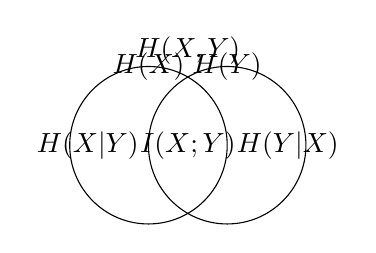
\begin{tikzpicture}
    \node at (0,1) {$H(X)$};
    \node at (1,1) {$H(Y)$};
    \node at (.5,1.2) {$H(X,Y)$};
    \node at (.5,0) {$I(X;Y)$};
    \draw (0,0) circle (1) node [left] {$H(X\vert Y)$};
    \draw (1,0) circle (1) node [right] {$H(Y\vert X)$};
\end{tikzpicture}
\begin{tikzpicture}
    \node at (0,1.4) {所有编码};
    \node at (0,1) {非奇异码};
    \draw (0,.4) circle (.9);
    \node at (0,.6) {唯一可解码};
    \draw (0,.2) circle (.7);
    \draw (0,0) circle (.5) node {瞬时码};
\end{tikzpicture}\\
\end{multicols*}
\end{document}